%%%%%%%%%%%%%%%%%%%%%%%%%%%%%%%%%%%%%%%%%%%%%%%%%%%%%%%%%%%%%%%%%%%%%%%%%%%%%%%%%%
\begin{frame}[fragile]\frametitle{}
\begin{center}
{\Large Linear Regression - Machine Learning Approach}
\end{center}
\end{frame}


%%%%%%%%%%%%%%%%%%%%%%%%%%%%%%%%%%%%%%%%%%%%%%%%%%%%%%%%%%%
\begin{frame}[fragile]\frametitle{Linear Regression: Which Line is Best?}
	\begin{itemize}
	\item We have multiple observations of inputs and an output
	\item Object: to find a model, ie a formulation, adhering to more or less all data points
	\item ie. to attempt to find the ``best'' line
	\item But, which line is the ``best''?
	\item The horizontal line is the worst, the benchmark. We need to beat that!!
	\end{itemize}
	
\begin{center}

\includegraphics[width=0.5\linewidth,keepaspectratio]{statq58}
\end{center}
	
\tiny{(Ref: StatQuest: Linear Models - Josh Starmer )}	
\end{frame}

%%%%%%%%%%%%%%%%%%%%%%%%%%%%%%%%%%%%%%%%%%%%%%%%%%%%%%%%%%%
\begin{frame}[fragile]\frametitle{Sum of Squared Errors for Benchmark Line}
	
\begin{center}

\includegraphics[width=0.8\linewidth,keepaspectratio]{statq59}
\end{center}
	
\tiny{(Ref: StatQuest: Linear Models - Josh Starmer )}	
	
\end{frame}

%%%%%%%%%%%%%%%%%%%%%%%%%%%%%%%%%%%%%%%%%%%%%%%%%%%%%%%%%%%
\begin{frame}[fragile]\frametitle{Sum of Squared Errors: Rotate a Little}

\begin{center}

\includegraphics[width=0.8\linewidth,keepaspectratio]{statq60}
\end{center}

Its better but is this best?

\tiny{(Ref: StatQuest: Linear Models - Josh Starmer )}	

\end{frame}

%%%%%%%%%%%%%%%%%%%%%%%%%%%%%%%%%%%%%%%%%%%%%%%%%%%%%%%%%%%
\begin{frame}[fragile]\frametitle{Sum of Squared Errors: Rotate a Bit More}
Rotated a bit more. Better?


\begin{center}

\includegraphics[width=0.8\linewidth,keepaspectratio]{statq61}
\end{center}

Its better but is this best?

\tiny{(Ref: StatQuest: Linear Models - Josh Starmer )}	

\end{frame}

%%%%%%%%%%%%%%%%%%%%%%%%%%%%%%%%%%%%%%%%%%%%%%%%%%%%%%%%%%%
\begin{frame}[fragile]\frametitle{Sum of Squared Errors: Rotate Too Far}
Why not rotate a whole lot!!


\begin{center}

\includegraphics[width=0.7\linewidth,keepaspectratio]{statq62}
\end{center}

No, we lost the BEST point somewhere in between. Whats that ``optimized'' point?

\tiny{(Ref: StatQuest: Linear Models - Josh Starmer )}	

\end{frame}

%%%%%%%%%%%%%%%%%%%%%%%%%%%%%%%%%%%%%%%%%%%%%%%%%%%%%%%%%%%
\begin{frame}[fragile]\frametitle{Optimization: Formulating the Problem}
To find the sweet spot ie the optimized point, lets put some formulation based on generic line equation.


\begin{center}

\includegraphics[width=0.7\linewidth,keepaspectratio]{statq63}
\end{center}



\tiny{(Ref: StatQuest: Linear Models - Josh Starmer )}	

\end{frame}

%%%%%%%%%%%%%%%%%%%%%%%%%%%%%%%%%%%%%%%%%%%%%%%%%%%%%%%%%%%
\begin{frame}[fragile]\frametitle{Optimization: The Least Squares Objective}
Mathematically \ldots

\begin{center}

\includegraphics[width=0.7\linewidth,keepaspectratio]{statq64}
\end{center}

Since we want the line that will give us the smallest sum of the squares of errors (SSE: Sum of Squared Errors), this method for finding the best values for ``a'' and ``b'' is called ``Least Squares''.

\tiny{(Ref: StatQuest: Linear Models - Josh Starmer )}	

\end{frame}

%%%%%%%%%%%%%%%%%%%%%%%%%%%%%%%%%%%%%%%%%%%%%%%%%%%%%%%%%%%
\begin{frame}[fragile]\frametitle{Optimization: The SSE Curve}
\begin{itemize}
\item If we plotted SSE for each rotated line the plot looks like.
\item We can see that SSE was high for the horizontal line, then came down as we started rotating the line, 
\item But started rising again, if we passed the sweet spot.
\end{itemize}

\begin{center}

\includegraphics[width=0.7\linewidth,keepaspectratio]{statq65}
\end{center}

\tiny{(Ref: StatQuest: Linear Models - Josh Starmer )}	

\end{frame}

% %%%%%%%%%%%%%%%%%%%%%%%%%%%%%%%%%%%%%%%%%%%%%%%%%%%%%%%%%%%
% \begin{frame}[fragile]\frametitle{Optimization (Recap)}
% \begin{itemize}
% \item If we plotted SSE for each rotated line the plot looks like. 
% \item We can see that SSE was high for the horizontal line, then came down as we started rotating the line, 
% \item But started rising again, if we passed the sweet spot.
% \end{itemize}

% \begin{center}
% 
\includegraphics[width=0.8\linewidth,keepaspectratio]{statq65}
% \end{center}

% Whats the Machine Learning way of finding the Sweet Spot? Its Gradient Decent!!

% \tiny{(Ref: StatQuest: Linear Models - Josh Starmer )}	

% \end{frame}

%%%%%%%%%%%%%%%%%%%%%%%%%%%%%%%%%%%%%%%%%%%%%%%%%%%%%%%%%%%
\begin{frame}[fragile]\frametitle{Optimization: Sliding Down the Curve}
\begin{itemize}
\item We need to get to the bottom point.
\item We can start at any (random) point, and SLIDE down to bottom.
\item SLIDING means going along slope. 
\item Slope is given by Derivative of the (SSE) function/curve, at the point 
\end{itemize}

\begin{center}

\includegraphics[width=0.7\linewidth,keepaspectratio]{statq66}
\end{center}

\tiny{(Ref: StatQuest: Linear Models - Josh Starmer )}	

\end{frame}

%%%%%%%%%%%%%%%%%%%%%%%%%%%%%%%%%%%%%%%%%%%%%%%%%%%%%%%%%%%
\begin{frame}[fragile]\frametitle{Optimization: Finding the Zero Slope}
\begin{itemize}
\item Slope starts decreasing from end, faster, then slower,
\item Reaches 0, horizontal, and then starts increasing again.
\item Need to find the ``0'' slope point.
\end{itemize}

\begin{center}

\includegraphics[width=0.24\linewidth,keepaspectratio]{statq67}

\includegraphics[width=0.24\linewidth,keepaspectratio]{statq68}

\includegraphics[width=0.24\linewidth,keepaspectratio]{statq69}

\includegraphics[width=0.24\linewidth,keepaspectratio]{statq70}
\end{center}

These different slopes mean different ``a'' parameters
\tiny{(Ref: StatQuest: Linear Models - Josh Starmer )}	

\end{frame}


%%%%%%%%%%%%%%%%%%%%%%%%%%%%%%%%%%%%%%%%%%%%%%%%%%%%%%%%%%%
\begin{frame}[fragile]\frametitle{Optimization: Gradient Descent Steps}

\begin{center}

\includegraphics[width=0.7\linewidth,keepaspectratio]{statq71}
\end{center}

\tiny{(Ref: StatQuest: Linear Models - Josh Starmer )}	

\end{frame}

%%%%%%%%%%%%%%%%%%%%%%%%%%%%%%%%%%%%%%%%%%%%%%%%%%%%%%%%%%%
\begin{frame}[fragile]\frametitle{Gradient Descent: the Slope, Precisely}
\adjustbox{valign=t}{%
\begin{minipage}{0.55\linewidth}
\begin{itemize}
\item First-order optimization algorithm.
\item Start at an arbitrary point on the SSE curve, repeatedly step in the downward direction, found by taking the negative of the gradient (the slope).
\item After several iterations, converge to the minimum. Here, that minimum is the $a, b$ (slope, intercept) that give the least error.
\item The learning rate $\alpha$ sets how big each downhill step is.
\end{itemize}
\end{minipage}%
}%
\hfill%
\adjustbox{valign=t}{%
\begin{minipage}{0.42\linewidth}
\begin{center}
\adjustbox{max width=\linewidth}{%
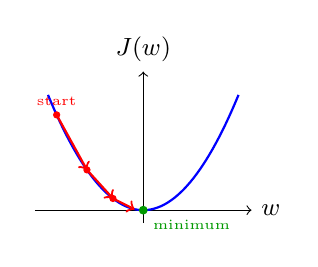
\begin{tikzpicture}[scale=0.55]
\draw[->] (-2.5,0) -- (2.5,0) node[right] {\small $w$};
\draw[->] (0,-0.3) -- (0,3.2) node[above] {\small $J(w)$};
\draw[thick, blue] plot[domain=-2.2:2.2, samples=60] (\x, {0.55*\x*\x});
\filldraw[red] (-2,2.2) circle (2pt) node[above] {\tiny start};
\draw[->, red, thick] (-2,2.2) -- (-1.3,0.93);
\filldraw[red] (-1.3,0.93) circle (2pt);
\draw[->, red, thick] (-1.3,0.93) -- (-0.7,0.27);
\filldraw[red] (-0.7,0.27) circle (2pt);
\draw[->, red, thick] (-0.7,0.27) -- (-0.2,0.02);
\filldraw[green!60!black] (0,0) circle (2.5pt) node[below right] {\tiny minimum};
\end{tikzpicture}}
\end{center}
\tiny{Each step moves opposite to the gradient (steepest descent); $\alpha$ sets the step size.}
\end{minipage}%
}
\end{frame}

%%%%%%%%%%%%%%%%%%%%%%%%%%%%%%%%%%%%%%%%%%%%%%%%%%%%%%%%%%%
\begin{frame}[fragile]\frametitle{Gradient Descent: the Update Rule}
For two parameters ($a$ and $b$, our slope and intercept), repeat until convergence:
\begin{align*}
a^{t+1} &= a^t - \alpha \frac{\partial J(a,b)}{\partial a}\\
b^{t+1} &= b^t - \alpha \frac{\partial J(a,b)}{\partial b}
\end{align*}
\begin{itemize}
\item Each partial derivative is the ``slope'' the earlier StatQuest slides pointed at, written out formally.
\item Convex bowl (one clean minimum): this always finds the bottom.
\item Non-convex surfaces: can get stuck in a local minimum, run from several starting points instead.
\end{itemize}

\begin{block}{Intuition}
This is the arithmetic behind ``sliding down the curve'': at every point, compute the slope, step a little opposite to it, repeat. Too large an $\alpha$ overshoots; too small is painfully slow.
\end{block}
\end{frame}

%%%%%%%%%%%%%%%%%%%%%%%%%%%%%%%%%%%%%%%%%%%%%%%%%%%%%%%%%%%
\begin{frame}[fragile]\frametitle{Stochastic Gradient Descent}
\begin{itemize}
\item Plain (``batch'') gradient descent computes the slope using every data point before taking one step.
\item Stochastic Gradient Descent instead uses a small random batch of data per step.
\item Computationally cheaper per step, and often converges faster in practice on large datasets.
\end{itemize}
\end{frame}


%%%%%%%%%%%%%%%%%%%%%%%%%%%%%%%%%%%%%%%%%%%%%%%%%%%%%%%%%%%
\begin{frame}[fragile]\frametitle{Optimization: Two Parameters, a Surface}
\begin{itemize}
\item For ``a'' and ``b'' both to be optimized, we will need 3D picture, as the Loss function would then take Z axis
\item It will be a Surface.
\item Derivative will be Partial, but the objective is the same, Bottom-most point. ie Minimum Loss function value
\end{itemize}

\begin{center}

\includegraphics[width=0.5\linewidth,keepaspectratio]{statq72}
\end{center}

The ``a'' and ``b'' coordinates corresponding to the bottom-most point give most minimum Loss. So it represents the ``best'' line.

\tiny{(Ref: StatQuest: Linear Models - Josh Starmer )}	

\end{frame}

%%%%%%%%%%%%%%%%%%%%%%%%%%%%%%%%%%%%%%%%%%%%%%%%%%%%%%%%%%%
\begin{frame}[fragile]\frametitle{Results}

\begin{center}

\includegraphics[width=0.7\linewidth,keepaspectratio]{statq73}
\end{center}

\tiny{(Ref: StatQuest: Linear Models - Josh Starmer )}	

\end{frame}


%%%%%%%%%%%%%%%%%%%%%%%%%%%%%%%%%%%%%%%%%%%%%%%%%%%%%%%%%%%
\begin{frame}[fragile]\frametitle{Example: Mouse Size }
\begin{itemize}
\item We have data points having mouse size and mouse weight
\item We wish to find mouse size given mouse weight.
\end{itemize}

\begin{center}

\includegraphics[width=0.7\linewidth,keepaspectratio]{statq74}
\end{center}

we use $R^2$ to find ``good-ness'' of fit (of line)

\tiny{(Ref: StatQuest: Linear Models - Josh Starmer )}	

\end{frame}



%%%%%%%%%%%%%%%%%%%%%%%%%%%%%%%%%%%%%%%%%%%%%%%%%%%%%%%%%%%%%%%%%%%%%%%%
\begin{frame}[fragile]\frametitle{Linear Regression for Complex Problems}
\adjustbox{valign=t}{%
\begin{minipage}{0.56\linewidth}%
\begin{itemize}
\item In real life, problems are far more complex than just one x and one y.
\item There could be many x's ie many inputs which decide the output
\item General formulation : Predicting quantitative response $y$ based on predictor variables $x$. Assumes linear relationship between $x$ and $y$
\end{itemize}
\adjustbox{max width=\linewidth}{$
y_i = \beta_0 + x_{1,i} \beta_1 + x_{2,i} \beta_2 + \cdots + x_{p,i} \beta_p + \epsilon_i
$}
\begin{itemize}
\item Objective is to find the parameters $\beta_j$ that minimize the squared residuals
\item There is no simple slope formula for each $\beta_j$, unlike the two-variable case.
\item The matrix formula $(X^TX)^{-1}X^Ty$ still holds, but inverting $X^TX$ gets impractical. So we solve it the machine learning way.
\end{itemize}
\end{minipage}%
}%
\hfill%
\adjustbox{valign=t}{%
\begin{minipage}{0.4\linewidth}%
\begin{center}
\adjustbox{max width=\linewidth}{%
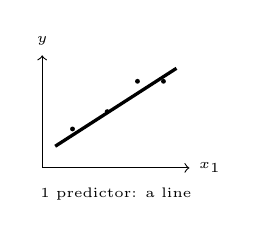
\begin{tikzpicture}[scale=0.55]
\draw[->] (0,0) -- (3.4,0) node[right,font=\tiny] {$x_1$};
\draw[->] (0,0) -- (0,2.6) node[above,font=\tiny] {$y$};
\draw[very thick] (0.3,0.5) -- (3.1,2.3);
\fill (0.7,0.9) circle (1.6pt);
\fill (1.5,1.3) circle (1.6pt);
\fill (2.2,2.0) circle (1.6pt);
\fill (2.8,2.0) circle (1.6pt);
\node[font=\tiny] at (1.7,-0.6) {1 predictor: a line};
\end{tikzpicture}}

\vspace{4pt}

\adjustbox{max width=\linewidth}{%
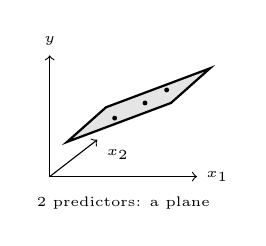
\begin{tikzpicture}[scale=0.55]
\draw[->] (0,0) -- (3.4,0) node[right,font=\tiny] {$x_1$};
\draw[->] (0,0) -- (0,2.8) node[above,font=\tiny] {$y$};
\draw[->] (0,0) -- (1.1,0.85) node[below right,font=\tiny] {$x_2$};
\draw[thick,fill=gray!20] (0.4,0.8) -- (2.8,1.7) -- (3.7,2.5) -- (1.3,1.6) -- cycle;
\fill (1.5,1.35) circle (1.6pt);
\fill (2.2,1.7) circle (1.6pt);
\fill (2.7,2.0) circle (1.6pt);
\node[font=\tiny] at (1.7,-0.6) {2 predictors: a plane};
\end{tikzpicture}}
\end{center}
\tiny{One predictor gives a line, two give a plane. Beyond that the fit still exists, we just cannot draw it.}
\end{minipage}%
}%
\end{frame}

%%%%%%%%%%%%%%%%%%%%%%%%%%%%%%%%%%%%%%%%%%%%%%%%%%%
\begin{frame}[fragile]\frametitle{Quick Check: Gradient Descent}
\begin{block}{Think About It}
The analytical formula $W = (X^TX)^{-1}X^Ty$ gives the exact best line in one shot. Gradient Descent only creeps towards it, one step at a time, and may never land exactly on it. So why is Gradient Descent the method that actually runs in practice?
\end{block}
\end{frame}

%%%%%%%%%%%%%%%%%%%%%%%%%%%%%%%%%%%%%%%%%%%%%%%%%%%%%%%%%%%%%%%%%%%%%%%%%%%%%%%%%%
\begin{frame}[fragile]\frametitle{Quick Check: Gradient Descent}
\begin{block}{Answer}
Because the formula requires inverting $X^TX$, and that becomes impossibly slow as the number of features grows, besides failing outright when two features are linearly dependent. Gradient Descent never inverts anything: it only needs the slope at the current point, so it scales to huge datasets. It also generalises, since the same walk-downhill idea trains models such as neural networks, where no closed-form formula exists at all. Being approximate is a price worth paying.
\end{block}
\end{frame}
